\item \points{2} {\bf Memory Augmented Neural Networks (MANN)     \cite{pmlr-v48-santoro16,DBLP:journals/corr/MishraRCA17}}

We will now be implementing few-shot classification using memory augmented neural networks (MANNs). The main idea of MANN is that the network should learn how to encode the first $K$ examples of each class into memory such that it can be used to accurately classify the $K+1$th example. See Figure \ref{mann} for a graphical representation of this process.

Data processing will be done as in SNAIL~\cite{DBLP:journals/corr/MishraRCA17}. Each set of labels and images are concatenated together, and the $N*K$ support set examples are sequentially passed through the network as shown in Fig. \ref{mann}. Then the query example of each class is fed through the network, \textbf{concatenated with 0 instead of the true label}. The loss is computed between the query set predictions and the ground truth labels, which is then backpropagated through the network. \textbf{Note}: The loss is \textit{only} computed on the set of $N$ query images, which comprise of the last examples from each character class. 

\begin{figure}
\centering
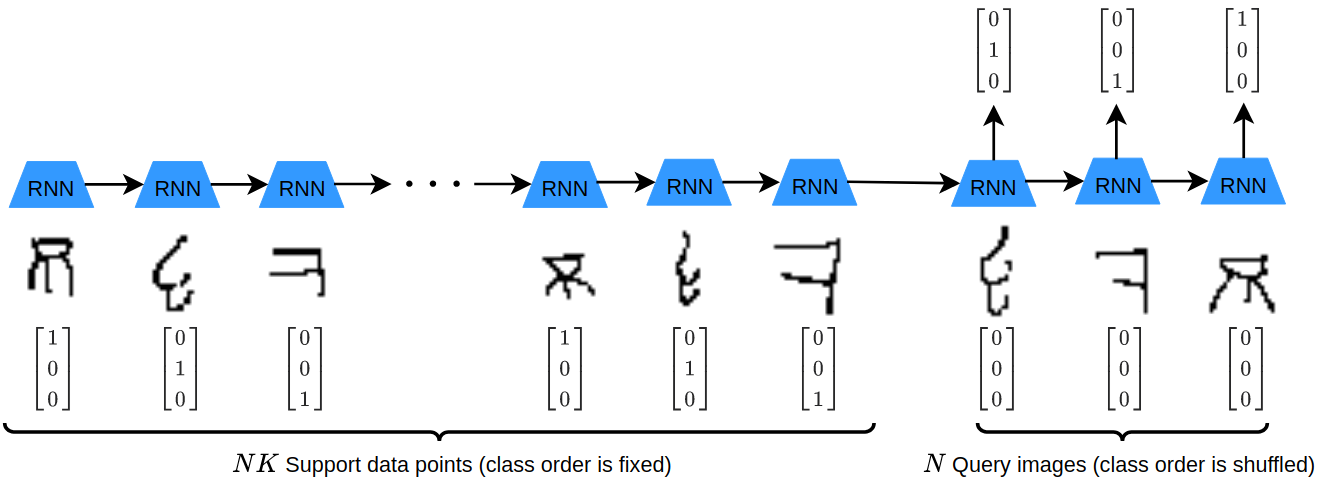
\includegraphics[width=\linewidth]{./figures/ps2seq}
\vspace{-9mm}
\caption{Feed $K$ labeled examples of each of $N$ classes through the memory-augmented network. Then feed final set of $N$ examples and optimize to minimize loss.}
\label{mann}
\end{figure}

\noindent In the \texttt{submission/mann.py} file:
\begin{enumerate}
    \item Fill in the \texttt{forward} function of the \texttt{MANN} class to take in image tensor of shape [$B, K+1, N, 784$] and a label tensor of shape [$B, K+1, N, N$] and output labels of shape [$B,K+1,N, N$]. The layers to use have already been defined for you in the \texttt{\_\_init\_\_} function. \textit{Hint: Remember to pass zeros, not the ground truth labels for the final $N$ examples.}
    \item  Fill in the function called \texttt{loss\_function} in the \texttt{MANN} class which takes as input the [$B,K+1,N, N$] labels and [$B,K+1,N, N$] predicted labels and computes \href{https://pytorch.org/docs/stable/generated/torch.nn.functional.cross_entropy.html#torch.nn.functional.cross_entropy}{the cross entropy loss} only on the $N$ test images. 
\end{enumerate}
\textbf{Note}: Both of the above functions will need to be backpropogated through, so they need to be written in PyTorch in a differentiable way.

\clearpage